\documentclass[12pt,a4paper]{article}
\usepackage{vkCourseML}
\usepackage{lipsum}
\usepackage{indentfirst}
\usepackage{tikz}
\usepackage{float}

\title{Машинное обучение, ФКН ВШЭ\\Семинар №17}
\author{}
\date{}

\newcommand{\ENC}{\text{ENC}}
\newcommand{\DEC}{\text{DEC}}

\begin{document}
\maketitle

\section{Машинное обучение на графах}

Активное развитие глубинного обучения в 2010-ых привело к появлению архитектур, специально разработанных для определенных типов данных. Например, сверточные нейронный сети являются общепризнанным стандартом для обработки изображений, а рекуррентные нейронные сети отлично подходят для работы с последовательностями. Тут конечно, стоит оговориться, что появление и активное распространение архитектуры трансформера немного стерло эти рамки, но подобное разделение до сих пор актуально при внедрении моделей на практике. Тем не менее, когда мы сталкиваемся с данными более сложной структуры, чем тексты или картинки, становится непонятно, как правильно обрабатывать их. Однако, очень многие данные можно представить как некоторый граф из вершин и связей между ними. По этой причине было бы разумно придумать методы машинного обучения, способные решать задачи на графах. Тут есть несколько возможных путей.

Первый вариант более сложный, но, как правило, наиболее эффективный. Он заключается в разработке методов, которые явно учитывают графовую структуру данных, например, это могут быть всякие разновидности графовых нейронных сетей, учитывающих связи между вершинами при вычислении активаций. В рамках этого семинара мы не будем фокусироваться на подобных алгоритмах ввиду их сложности и специфичности. Другой вариант подойдет нам больше, поскольку его проще завести ''из коробки''. Мы можем решить задачу обучения представлений на графе, а полученные представления использовать в качестве признакового описания графов и обучать на них уже знакомые нам алгоритмы: линейные модели или градиентные бустинги. Такой пайплайн обработки скорее всего будет неплохим бейзлайном для нашей графовой задачи.

Задачи на графах можно разделить на две категории:
\begin{itemize}
    \item Объектом является вершина графа (\emph{node-focused tasks}). В этом случае мы хотим изучать структурные свойства вершины относительно других вершин. В качестве примеров задач приведем \textbf{классификацию вершин} (поиск хабов в транспортных сетях), \textbf{предсказание связей} (предсказание взаимодействия между белками), \textbf{рекомендацию вершин} (поиск возможных друзей в социальных сетях).

    \item Объектом является подграф или весь граф целиком (\emph{graph-focused tasks}). Примерами таких задач будут \textbf{классификация графов} (предсказание токсичности молекулы), \textbf{генерация графов} (получение молекул белков с желаемыми свойствами), \textbf{оценивание глобальных свойств графа} (предсказание химических/физических характеристик молекулы).
\end{itemize}

\section{Представления для вершин}

Начнем с обсуждения методов для обучения векторных представлений для вершин одного графа. Нам бы хотелось, чтобы вектор-эмбеддинг включал в себя информацию о структурной роли вершины, например, о расстоянии от этой вершины до всех остальных. Введем обозначения: пусть у нас есть граф $\mathcal{G} = (\mathcal{V}, \mathcal{E})$, где $\mathcal{V} = \{v_i\}_{i=1}^{|\mathcal{V}|}$ --- множество вершин, а $\mathcal{E}: \mathcal{V}\times\mathcal{V}\to\mathbb{R}_{\ge 0}$ --- ребра с неотрицательными весами. Зададим некоторую функцию похожести между вершинами $s_{\mathcal{G}}: \mathcal{V}\times\mathcal{V}\to\mathbb{R}$. В простейшем случае можно взять $s_{\mathcal{G}}(v_i, v_j)=1$, если $v_i$ и $v_j$ соединены ребром и $s_{\mathcal{G}}(v_i, v_j)=0$ иначе. Либо можно использовать формулу, зависящую от растояния между вершинами, например:
$$
s_{\mathcal{G}}(v_i, v_j) = \exp\left(-\frac{d_{\mathcal{G}}(v_i, v_j)}{\tau}\right),
$$

\noindent
где $d_{\mathcal{G}}(v_i, v_j)$ --- расстояние между вершинами $v_i$ и $v_j$, а $\tau$ --- гиперпараметр. Заметим, что в этом случае похожесть вершины на саму себя равна единице, поскольку $d_{\mathcal{G}}(v_i, v_i)=0$, а если между двумя вершинами не существует пути, то получаем $d_{\mathcal{G}}(v_i, v_i)=+\infty$ и $s_{\mathcal{G}}(v_i, v_j)=0$. Третий вариант задать функцию похожести --- оценить вероятность перехода из одной вершины в другую при случайном блуждании по графу. О том, как это сделать, мы поговорим далее.

\subsection{node2vec}

Мы рассмотрим методы на основе принципа энкодер--декодер. Пусть энкодер преобразует наши вершины в векторы некоторой размерности $d$, $\ENC: \mathcal{V} \to \mathbb{R}^d, \ENC(v_i)=z_i$, а декодер принимает два векторных представления и пытается приблизить функцию похожести сответствующих вершин, $\DEC: \mathbb{R}^d \times \mathbb{R}^d \to \mathbb{R}, \DEC(z_i, z_j)\approx s_{\mathcal{G}}(v_i, v_j)$. Для того, чтобы обучить всю эту конструкцию, мы можем взять удобную нам функцию потерь $\mathcal{L}(\cdot, \cdot)$ (например, MSE или кросс-энтропию) и проминизировать ее по параметрам энкодера и декодера:
$$
\sum_{v_i, v_j \in \mathcal{V}} \mathcal{L} \bigg(\DEC\Big(\ENC(v_i), \ENC(v_j)\Big), s_{\mathcal{G}}(v_i, v_j)\bigg) \to \min_{\ENC, \DEC}
$$

\noindent
Обученные векторы $z = \ENC(v)$ и будут искомыми представлениями. В простейшем случае в качестве энкодера мы можем взять матрицу размерности $|\mathcal{V}| \times d$, то есть каждой вершине будет поставлен в соответствие некоторый вектор из $\mathbb{R}^d$. В роли декодера часто используют обычное скалярное произведение, $\DEC(z_i, z_j) = z_i^T z_j$. Но мы рассмотрим более продвинутый метод, который называется \emph{node2vec}.

Главная особенность метода --- использование вероятности случайного блуждания в качестве функции похожести. Пусть вероятность попасть из вершины $v_i$ в вершину $v_j$ при случайном блужданиии равна $p(v_j|v_i)$. Мы хотим обучить такие векторы-эмбеддинги $z$, что выполняется:
$$
p(v_j|v_i) \approx \frac{e^{z_j^T z_i}}{\sum_k e^{z_k^T z_i}} = \DEC(z_i, z_j)
$$

\noindent
Иными словами, в качестве декодера мы будем использовать оператор Softmax от скалярных произведений векторных представлений. Здесь возникает следующая проблема: посчитать $p(v_j|v_i)$ аналитически мы можем только для очень простых графов, но для реальных данных это едва ли возможно. Тем не менее, мы можем запустить случайное блуждания по графу и оценить, какие вершины чаще встречаются на одном пути. Фактически, node2vec --- это модель \emph{skip-gram word2vec}, в которой словами являются вершины графа, а предложениями --- случайные пути в этом графе. Так что если читатель знаком с последней, то следующие абзацы станут для него повторением уже пройденного.

\begin{center}
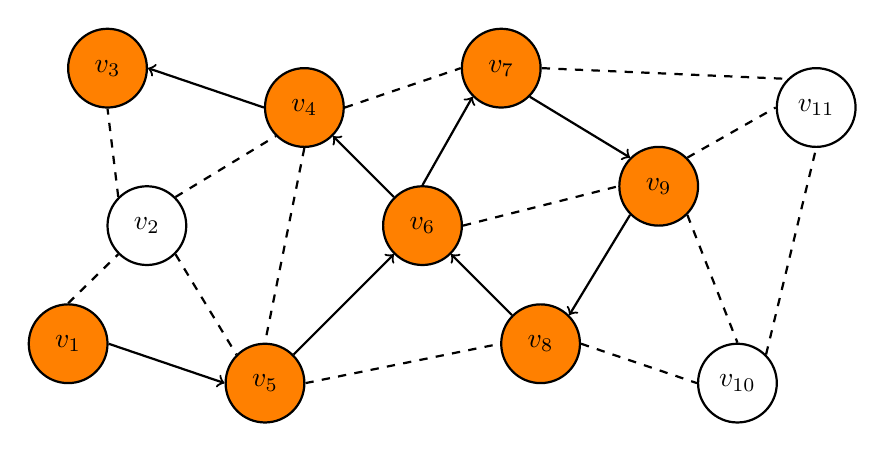
\begin{tikzpicture}[
roundnode/.style={circle, draw=black, thick, minimum size=10mm}
]

\node[roundnode, fill=orange] at (-2, 4) (3) {$v_3$};
\node[roundnode, fill=orange] at (0.5, 3.5) (4) {$v_4$};
\node[roundnode, fill=orange] at (-2.5, 0.5) (1) {$v_1$};
\node[roundnode] at (-1.5, 2) (2) {$v_2$};
\node[roundnode, fill=orange] at (0, 0) (5) {$v_5$};
\node[roundnode, fill=orange] at (2, 2) (6) {$v_6$};
\node[roundnode, fill=orange] at (3.5, 0.5) (8) {$v_8$};
\node[roundnode, fill=orange] at (5, 2.5) (9) {$v_9$};
\node[roundnode] at (6, 0) (10) {$v_{10}$};
\node[roundnode, fill=orange] at (3, 4) (7) {$v_7$};
\node[roundnode] at (7, 3.5) (11) {$v_{11}$};

\draw[->, thick] (1.east) -- (5.west);
\draw[->, thick] (5.north east) -- (6.south west);
\draw[->, thick] (6.north) -- (7.south west);
\draw[->, thick] (7.south east) -- (9.north west);
\draw[->, thick] (9.south west) -- (8.north east);
\draw[->, thick] (8.north west) -- (6.south east);
\draw[->, thick] (6.north west) -- (4.south east);
\draw[->, thick] (4.west) -- (3.east);

\draw[-, dashed, thick] (1.north) -- (2.south west);
\draw[-, dashed, thick] (2.north west) -- (3.south);
\draw[-, dashed, thick] (2.north east) -- (4.south west);
\draw[-, dashed, thick] (2.south east) -- (5.north west);
\draw[-, dashed, thick] (4.south) -- (5.north);
\draw[-, dashed, thick] (4.east) -- (7.west);
\draw[-, dashed, thick] (5.east) -- (8.west);
\draw[-, dashed, thick] (6.east) -- (9.west);
\draw[-, dashed, thick] (7.east) -- (11.north west);
\draw[-, dashed, thick] (8.east) -- (10.west);
\draw[-, dashed, thick] (9.north east) -- (11.west);
\draw[-, dashed, thick] (9.south east) -- (10.north);
\draw[-, dashed, thick] (10.north east) -- (11.south);
\end{tikzpicture}
\end{center}

Рассмотрим в качестве примера граф выше и случайный путь $W$ по нему. Пусть $S=[v_1, v_5, v_6, v_7, v_9, v_8, v_6, v_4, v_3]$. Теперь зафиксируем некоторый размер окна $w$, например, $w=2$, и для каждой вершины, которая встретилась на пути посмотрим на окно с центром в ней. Для начальной вершины $v_1$ окно будет выглядеть как $[\underline{v_1}, v_5, v_6]$, для первого вхождения $v_6$ получим $[v_1, v_5, \underline{v_6}, v_7, v_9]$, а для второго --- $[v_9, v_8, \underline{v_6}, v_4, v_3]$. Далее, для каждого окна выпишем пары вида (центр окна, другое упоминание вершины в окне), напимер для окна $[v_1, v_5, \underline{v_6}, v_7, v_9]$ получим пары $(v_6, v_1)$, $(v_6, v_5)$, $(v_6, v_7)$, $(v_6, v_9)$. Назовем такие пары $(v_i, v_j)$ позитивными и постараемся собрать таких как можно больше, увеличивая длину и число запусков случайного блуждания. Теперь, чтобы обучить векторы-эмбеддинги, мы будем минимизировать следующий функционал:
$$
\mathcal{L} = \sum_{(v_i, v_j)} -\log \big(\DEC(z_i, z_j)\big) = \sum_{(v_i, v_j)} \Big(-z_j^T z_i + \log \sum_k e^{z_k^T z_i} \Big) \to \min_{z}
$$

Единственная проблема, которую осталось решить --- подсчет знаменателя в операторе Softmax, который имеет линейную сложность по числу вершин, что будет работать очень медленно для больших графов. Чтобы избежать это недоразумение, пользуются трюком под названием \emph{negative sampling} --- вместо подсчета всей суммы экспонент мы можем случайно выбрать несколько негативных пар (то есть вершин, которые не попали в окно с центром в $v_i$) и с их помощью оценить знаменатель, то есть теперь мы считаем знаменатель за константное время вместо линейного.

Обученные методом node2vec векторные представления будут содержать информацию о близости вершин с точки зрения случайного блуждания. Но случайное блуждание случайному блужданию рознь. Мы можем захотеть, чтобы наши эмбеддинги хорошо описывали локальную окрестность каждой вершины, тогда будет разумно взять случайное блуждание, похожее на обход графа в ширину. Или наоборот, мы можем захотеть пути, которые пробегаются по всему графу, не застревая в одном месте, тогда было бы уместно рассмотреть обход в глубину. Авторы node2vec вводят два гиперпараметра $p$ и $q$, которые позволяют переключаться между этими двумя режимами. Посмотрим на картинку:

\begin{center}
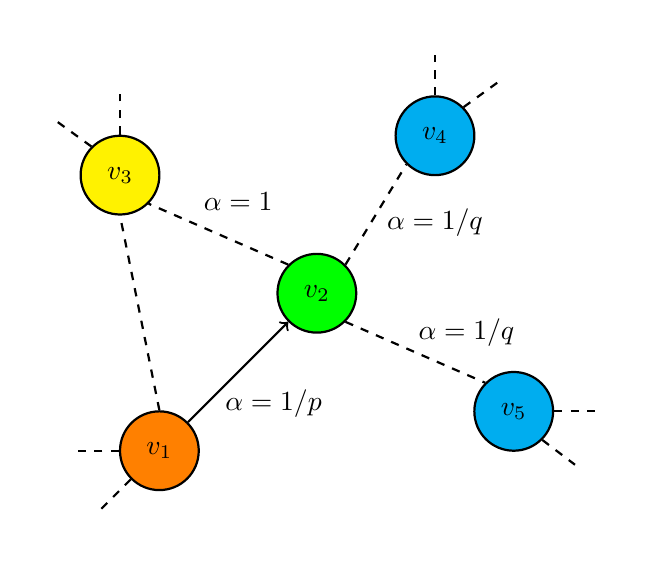
\begin{tikzpicture}[
roundnode/.style={circle, draw=black, thick, minimum size=10mm},
emptynode/.style={circle, draw=white}
]

\node[roundnode, fill=orange] at (0, 0) (1) {$v_1$};
\node[roundnode, fill=green] at (2, 2) (2) {$v_2$};
\node[roundnode, fill=yellow] at (-0.5, 3.5) (3) {$v_3$};
\node[roundnode, fill=cyan] at (3.5, 4) (4) {$v_4$};
\node[roundnode, fill=cyan] at (4.5, 0.5) (5) {$v_5$};

\node[emptynode] at (-1.2, 0) (1a) {};
\node[emptynode] at (-0.9, -0.9) (1b) {};
\node[emptynode] at (-1.5, 4.2) (3a) {};
\node[emptynode] at (-0.5, 4.7) (3b) {};
\node[emptynode] at (3.5, 5.2) (4a) {};
\node[emptynode] at (4.5, 4.7) (4b) {};
\node[emptynode] at (5.7, 0.5) (5a) {};
\node[emptynode] at (5.4, -0.3) (5b) {};

\draw[->, thick] (1.north east) -- (2.south west);
\draw[-, dashed, thick] (1.north) -- (3.south);
\draw[-, dashed, thick] (2.north west) -- (3.south east);
\draw[-, dashed, thick] (2.north east) -- (4.south west);
\draw[-, dashed, thick] (2.south east) -- (5.north west);

\draw[-, dashed, thick] (1.west) -- (1a.east);
\draw[-, dashed, thick] (1.south west) -- (1b.north east);
\draw[-, dashed, thick] (3.north west) -- (3a.east);
\draw[-, dashed, thick] (3.north) -- (3b.south);
\draw[-, dashed, thick] (4.north) -- (4a.south);
\draw[-, dashed, thick] (4.north east) -- (4b.west);
\draw[-, dashed, thick] (5.east) -- (5a.west);
\draw[-, dashed, thick] (5.south east) -- (5b.north west);

\node[below] at (1.45, 0.9) {$\alpha = 1/p$};
\node[below] at (3.9, 1.8) {$\alpha = 1/q$};
\node[below] at (3.5, 3.2) {$\alpha = 1/q$};
\node[below] at (1, 3.4) {$\alpha = 1$};

\end{tikzpicture}
\end{center}

\noindent
Допустим, на очередном шаге блуждания мы попали из вершины $v_1$ в вершину $v_2$. Чтобы определить вероятности перехода в соседние вершины, зададим веса ребрам $\alpha$:
\begin{enumerate}
    \item Для ребра, ведущего обратно, положим $\alpha = 1/p$.
    \item Для общих соседей предыдущей и текущей вершины положим $\alpha=1$.
    \item Для всех остальных вершин положим $\alpha = 1/q$.
\end{enumerate}

\noindent
Итоговая вероятность для ребра получаются как его вес, деленный на сумму всех весов ребер, выходящих из $v_2$. Проанализируем, что у нас получилось. Гиперпараметр $p$ контролирует вероятность возврата в предыдущую вершину. Чем больше $p$, тем больше мы будем посещать новые вершины вместо возврата обратно. Гиперпараметр $q$ регулирует уклон в сторону обхода в глубину/в ширину. Чем больше $q$, тем меньше вероятность покинуть соседей $v_1$, то есть мы больше склонны к обходу в ширину. И наоборот, чем меньше $q$, тем больше наше блуждание похоже на обход в глубину. Да, такая постановка дает нам два новых гиперпараметра, которые нужно подбирать, но делает модель гораздо более гибкой с точки зрения информации, которая сохраняется в эмбеддингах. 

Обсудим теперь, какие плюсы и минусы есть у метода node2vec. Среди достоинств можно выделить гибкость модели: мы можем выбирать, какую именно информацию заложить в эмбеддинги. Кроме того, модель радует своей простотой: пусть мы и обсудили много подробностей про случайные блуждания на графах, учим-то мы только саму матрицу эмбеддингов. В связи с ней же появляются следующие недостатки: мы не сможем создавать векторные представления для новых вершин, а также у нас нет никаких общих параметров для разных вершин, что может привести к переобучению. Более того, мы не используем метаданные, которые могут содержаться в вершинах. Далее мы поговорим про другие алгоритмы, которые исправляют минусы node2vec.

\subsection{Neighborhood autoencoder}

Попробуем немного видоизменить наш подход. Для начала поставим в соответствие каждой вершине вектор, состоящий из значений функции похожести на все остальные вершины: $v_i \mapsto s_i, s_{ij} = s_{\mathcal{G}}(v_i, v_j)$. Мы получили очень длинный вектор (его размер равен числу вершин в графе), к которому можно применить классические алгоритмы понижения размерности, например, PCA или что-нибудь нелинейное вроде автоэнкодера (это такая архитектура нейронной сети, содержащая ''бутылочное горлышко''). В итоге наша модель будет выглядеть так: $z_i = \ENC(s_i), \DEC(z_i) \approx s_i$. Учить ее можно, например, с помощью MSE:
$$
\sum_{i} \Big\|\DEC\big(\ENC(s_i)\big) - s_i\Big\|^2 \to \min_{\ENC, \DEC}
$$

В таком подходе параметры модели будут общими для всех вершин. Тем не менее, мы все еще не умеем генерировать эмбеддинги для новых вершин и не используем метаданные, содержащиеся в вершинах. Следующий метод исправляет и эти недостатки. 

\subsection{Neighborhood aggregation}

Попробуем придумать такой метод, который будет одновременно использовать структуру графа, учитывать метаданные, а также подойдет для генерации эмбеддингов для новых вершин. Для этого подойдет идея \emph{neighborhood aggregation}: для каждой вершины мы будем агрегировать признаки ее соседей и некоторым образом комбинировать с признаками самой вершины. Более подробно, алгоритм выглядит так:
\begin{enumerate}
    \item Начинаем с того, что у каждой вершины есть некоторый вектор с признаками (исходно можно взять метаданные вершин).
    \item Для каждой вершины агрегируем признаки ее соседей (в простейшем случае просто усредняем их).
    \item Комбинируем вектор признаков вершины и вектор признаков соседей (в простейшем случае конкатенируем их).
    \item К комбинированному вектору применяем линейное преобразование $W$ и нелинейную функцию $\sigma$. Получаем новые векторы признаков для каждой вершины.
    \item Теперь последовательно повторяем шаги 2--4 $K$ раз (с разными матрицами весов $W_k$ для $k=1,\dots, K$).
\end{enumerate}

\begin{figure}[H]
\centering
\begin{tikzpicture}[
roundnode/.style={circle, draw=black, thick, minimum size=3mm}
]
\node[roundnode] at (0, 0) (1) {};
\node[roundnode, fill=cyan] at (-0.4, 1.5) (2) {};
\node[roundnode, fill=cyan] at (1.5, -0.7) (3) {};
\node[roundnode, fill=cyan] at (-1.2, -0.9) (4) {};
\node[roundnode, fill=blue] at (0.5, 3) (5) {};
\node[roundnode, fill=blue] at (-1.5, 2.6) (6) {};
\node[roundnode, fill=blue] at (3.3, -0.4) (7) {};
\node[roundnode, fill=blue] at (2.8, -1.8) (8) {};
\node[roundnode, fill=blue] at (-2.7, -0.7) (9) {};
\node[roundnode, fill=blue] at (-2.3, -2) (10) {};

\draw[-, thick] (1.north) -- (2.south);
\draw[-, thick] (1.east) -- (3.north west);
\draw[-, thick] (1.south west) -- (4.north east);
\draw[-, thick] (2.north east) -- (5.south west);
\draw[-, thick] (2.north west) -- (6.south east);
\draw[-, thick] (3.east) -- (7.west);
\draw[-, thick] (3.south east) -- (8.north west);
\draw[-, thick] (4.west) -- (9.east);
\draw[-, thick] (4.south west) -- (10.north east);

\node[below] at (0.8, 1.2) {$\begin{bmatrix}1 \\ -1\end{bmatrix}$};
\node[below] at (-1, 1.8) {$\begin{bmatrix}0 \\ 1\end{bmatrix}$};
\node[below] at (0.75, -0.5) {$\begin{bmatrix}2.5 \\ 3\end{bmatrix}$};
\node[below] at (-1.1, -1.2) {$\begin{bmatrix}0.5 \\ 2\end{bmatrix}$};
\node[below] at (0, -2.7) {(1) Исходные векторы признаков};
\end{tikzpicture}
\hfill
\begin{tikzpicture}[
roundnode/.style={circle, draw=black, thick, minimum size=3mm}
]
\node[roundnode] at (0, 0) (1) {};
\node[roundnode, fill=cyan] at (-0.4, 1.5) (2) {};
\node[roundnode, fill=cyan] at (1.5, -0.7) (3) {};
\node[roundnode, fill=cyan] at (-1.2, -0.9) (4) {};
\node[roundnode, fill=blue] at (0.5, 3) (5) {};
\node[roundnode, fill=blue] at (-1.5, 2.6) (6) {};
\node[roundnode, fill=blue] at (3.3, -0.4) (7) {};
\node[roundnode, fill=blue] at (2.8, -1.8) (8) {};
\node[roundnode, fill=blue] at (-2.7, -0.7) (9) {};
\node[roundnode, fill=blue] at (-2.3, -2) (10) {};

\draw[<-, dashed, thick] (1.north) -- (2.south);
\draw[<-, dashed, thick] (1.east) -- (3.north west);
\draw[<-, dashed, thick] (1.south west) -- (4.north east);
\draw[-, thick] (2.north east) -- (5.south west);
\draw[-, thick] (2.north west) -- (6.south east);
\draw[-, thick] (3.east) -- (7.west);
\draw[-, thick] (3.south east) -- (8.north west);
\draw[-, thick] (4.west) -- (9.east);
\draw[-, thick] (4.south west) -- (10.north east);

\node[below] at (0.8, 1.2) {$\begin{bmatrix}1 \\ -1\end{bmatrix}$};
\node[below] at (-1, 1.8) {$\begin{bmatrix}0 \\ 1\end{bmatrix}$};
\node[below] at (0.75, -0.5) {$\begin{bmatrix}2.5 \\ 3\end{bmatrix}$};
\node[below] at (-1.1, -1.2) {$\begin{bmatrix}0.5 \\ 2\end{bmatrix}$};
\node[below] at (2.6, 2.7) {$\scriptstyle \textcolor{purple}{
\begin{bmatrix}
1 \\ 2
\end{bmatrix}} = \cfrac{1}{3} \bigg(
\begin{bmatrix}0 \\ 1\end{bmatrix} + 
\begin{bmatrix}2.5 \\ 3\end{bmatrix} + 
\begin{bmatrix}0.5 \\ 2\end{bmatrix}
\bigg)
$};

\node[below] at (0, -2.7) {(2) Агрегируем признаки соседей};
\end{tikzpicture}
\end{figure}

\begin{figure}[H]
\centering
\begin{tikzpicture}[
roundnode/.style={circle, draw=black, thick, minimum size=3mm}
]
\node[roundnode] at (0, 0) (1) {};
\node[roundnode, fill=cyan] at (-0.4, 1.5) (2) {};
\node[roundnode, fill=cyan] at (1.5, -0.7) (3) {};
\node[roundnode, fill=cyan] at (-1.2, -0.9) (4) {};
\node[roundnode, fill=blue] at (0.5, 3) (5) {};
\node[roundnode, fill=blue] at (-1.5, 2.6) (6) {};
\node[roundnode, fill=blue] at (3.3, -0.4) (7) {};
\node[roundnode, fill=blue] at (2.8, -1.8) (8) {};
\node[roundnode, fill=blue] at (-2.7, -0.7) (9) {};
\node[roundnode, fill=blue] at (-2.3, -2) (10) {};

\draw[-, thick] (1.north) -- (2.south);
\draw[-, thick] (1.east) -- (3.north west);
\draw[-, thick] (1.south west) -- (4.north east);
\draw[-, thick] (2.north east) -- (5.south west);
\draw[-, thick] (2.north west) -- (6.south east);
\draw[-, thick] (3.east) -- (7.west);
\draw[-, thick] (3.south east) -- (8.north west);
\draw[-, thick] (4.west) -- (9.east);
\draw[-, thick] (4.south west) -- (10.north east);

\node[below] at (0.8, 2.25) {$
\textcolor{blue}{\begin{bmatrix}
1 \\ -1 \\ 1 \\ 2
\end{bmatrix}}
$};
\node[below] at (2.25, 2.3) {$\leftarrow
\begin{bmatrix}
1 \\ -1
\end{bmatrix}
$};
\node[below] at (2.25, 1.2) {$\textcolor{purple}{\leftarrow
\begin{bmatrix}
1 \\ 2
\end{bmatrix}}
$};
\node[below] at (0, -2.7) {(3) Комбинируем векторы признаков};
\end{tikzpicture}
\hfill
\begin{tikzpicture}[
roundnode/.style={circle, draw=black, thick, minimum size=3mm}
]
\node[roundnode] at (0, 0) (1) {};
\node[roundnode, fill=cyan] at (-0.4, 1.5) (2) {};
\node[roundnode, fill=cyan] at (1.5, -0.7) (3) {};
\node[roundnode, fill=cyan] at (-1.2, -0.9) (4) {};
\node[roundnode, fill=blue] at (0.5, 3) (5) {};
\node[roundnode, fill=blue] at (-1.5, 2.6) (6) {};
\node[roundnode, fill=blue] at (3.3, -0.4) (7) {};
\node[roundnode, fill=blue] at (2.8, -1.8) (8) {};
\node[roundnode, fill=blue] at (-2.7, -0.7) (9) {};
\node[roundnode, fill=blue] at (-2.3, -2) (10) {};

\draw[-, thick] (1.north) -- (2.south);
\draw[-, thick] (1.east) -- (3.north west);
\draw[-, thick] (1.south west) -- (4.north east);
\draw[-, thick] (2.north east) -- (5.south west);
\draw[-, thick] (2.north west) -- (6.south east);
\draw[-, thick] (3.east) -- (7.west);
\draw[-, thick] (3.south east) -- (8.north west);
\draw[-, thick] (4.west) -- (9.east);
\draw[-, thick] (4.south west) -- (10.north east);

\node[below] at (2.1, 2.25) {$
\begin{bmatrix}
    0.5 \\ 0.2
\end{bmatrix} =
\textcolor{brown}{\sigma \bigg(W \cdot} 
\textcolor{blue}{\begin{bmatrix}
1 \\ -1 \\ 1 \\ 2
\end{bmatrix}}\textcolor{brown}{\bigg)}
$};
\node[below] at (0, -2.7) {(4) Вычисляем новые векторы признаков};
\end{tikzpicture}
\end{figure}

Фактически, мы получили полносвязную нейронную сеть, в которой связи между нейронами зависят от связей между вершинами в графе. Осталось обсудить, как именно учить такую модель, потому что параметры $\{W_k\}_{k=1}^K$ остаются ненастроенными. Делать это мы будем, разумеется, с помощью градиентного спуска (все использованные нами преобразования были дифференцируемыми), а в качестве функции потерь можно взять любую, из описанных выше, например, приближение некоторой функции похожести вершин или подход со случайными блужданиями, использованный в node2vec.

По сути, neighborhood aggregation --- это не что иное, как более продвинутый энкодер для генерации эмбеддингов. Он использует метаданные вершин, а также позволяет обрабатывать новые вершины, которые не встречались в обучающей выборке (мы точно так же можем провернуть шаги алгоритма для новых вершин, просто веса $W_k$ уже будут обученными).

Отдельно стоит упомянуть гиперпараметр глубины $K$: чем он больше, тем более широкая окрестность вершины влияет на ее векторное представление. За это приходится платить большим временем обработки и возможным переобучением засчет увеличения числа параметров (хотя, гипотетически, никто не запрещает нам брать одинаковые матрицы линейных преобразований на каждом шаге $W_k = W$, тогда у модели будут разделяемые параметры).

\section{Представления для графов}

Мы максимально подробно обсудили, как генерировать векторные представления для вершин графа. Остается вопрос, а как же нам кодировать весь граф целиком? Векторные представления для графа можно получить, скомбинировав представления для его вершин. Тут, опять же, есть несколько опций на выбор. В качестве самой простой усреднение эмбеддингов вершин:
$$
z_{\mathcal{G}} = \frac{1}{|\mathcal{V}|} \sum_{v \in \mathcal{V}} z_v
$$

\noindent
Либо же можно составить последовательность из эмбеддингов вершин и дальше обрабатывать ее, например, рекуррентными нейронными сетями:
$$
z_{\mathcal{G}} = (z_1, \dots, z_{\mathcal{V}})
$$

\noindent
В конце концов, можно использовать более продвинутые графовые нейронные сети, но их обсуждение выходит за рамки этого семинара.

\begin{thebibliography}{}
\bibitem{zhang}
    \emph{Ziwei Zhang, Peng Cui and Wenwu Zhu},
    Deep Learning on Graphs: A Survey, 2018

\bibitem{hamilton}
    \emph{William L. Hamilton, Rex Ying and Jure Leskovec},
    Representation Learning on Graphs: Methods and Applications, 2017

\bibitem{grover}
    \emph{Aditya Grover and Jure Leskovec},
    node2vec: Scalable Feature Learning for Networks, 2016

\bibitem{hamilton2}
    \emph{William L. Hamilton, Rex Ying and Jure Leskovec}
    Inductive Representation Learning on Large Graphs, 2017
\end{thebibliography}

\end{document}
